\documentclass[french]{standalone}
\usepackage{babel}
\usepackage{tkz-fct}
\usepackage{tkz-euclide}
\usepackage{color}
\usepackage{numprint}

\renewcommand*\familydefault{\sfdefault}
\usepackage{sansmath}
\sansmath
\definecolor{gray75}{gray}{0.75}

\begin{document}
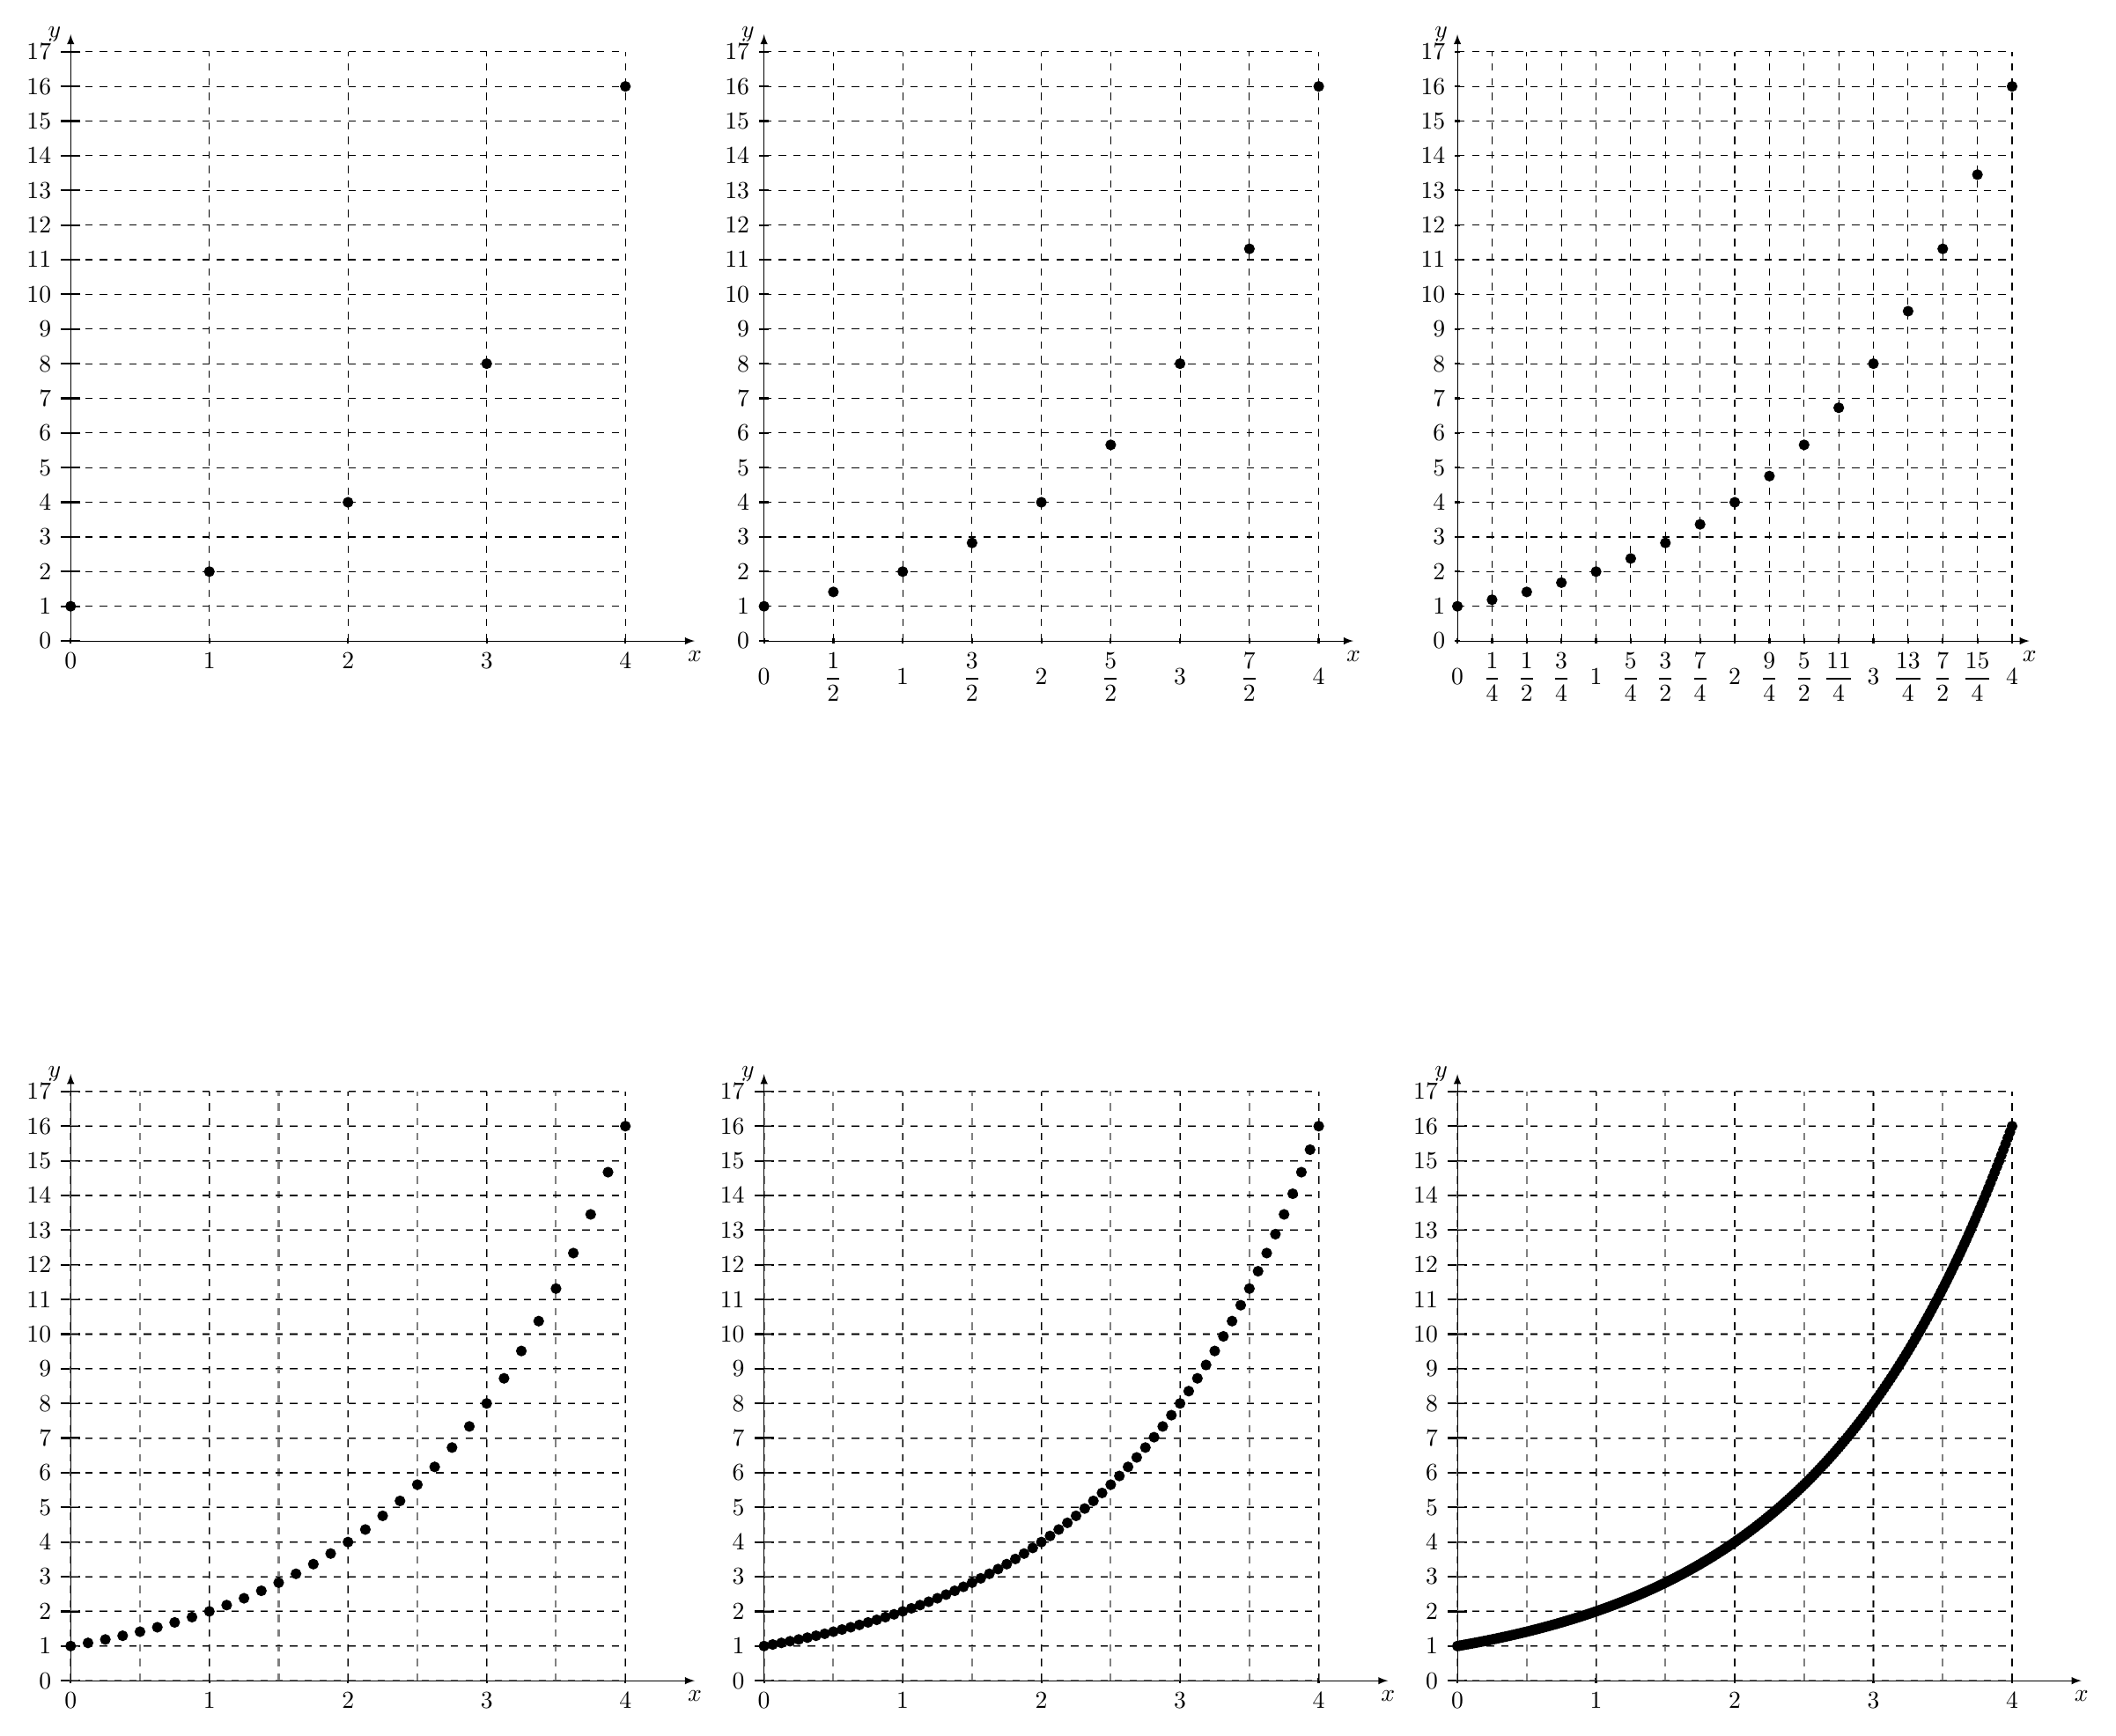
\begin{tikzpicture}[xscale=2,yscale=0.5]
  \tkzInit[xmin=0,xmax=4,ymin=0,ymax=17, ystep=1, xstep=1]
\tkzAxeY
\tkzDrawX
\tkzLabelX
   \begin{scope}[dashed]
     \tkzGrid[color=black]
   \end{scope}
\tkzSetUpPoint[size = 4]
\global\edef\tkzFctLast{(exp(x*ln(2)))}
\foreach \va in {0, 1,...,4}{%
  \tkzDefPointByFct[draw](\va)
}
  \begin{scope}[xscale=0.5,xshift=10cm]

\tkzInit[xmin=0,xmax=4,ymin=0,ymax=17, ystep=1, xstep=0.5]
\tkzAxeY
\tkzDrawX
\tkzLabelX[frac=2,below = 8pt]
   \begin{scope}[dashed]
     \tkzGrid[color=black]
   \end{scope}
\tkzSetUpPoint[size = 4]
\global\edef\tkzFctLast{(exp(x*ln(2)))}
\foreach \va in {0,0.5, 1, 1.5,...,4}{%
  \tkzDefPointByFct[draw](\va)
}
  \end{scope}
\begin{scope}[xscale=0.25,xshift=40cm]
  \tkzInit[xmin=0,xmax=4,ymin=0,ymax=17, ystep=1, xstep=0.25]
  \tkzAxeY
  \tkzDrawX
  \tkzLabelX[frac=4,below = 8pt]
     \begin{scope}[dashed]
       \tkzGrid[color=black]
     \end{scope}
  \tkzSetUpPoint[size = 4]
  \global\edef\tkzFctLast{(exp(x*ln(2)))}
  \foreach \va in {0,0.25,0.5,0.75, 1,...,4}{%
    \tkzDefPointByFct[draw](\va)
  }
\end{scope}
\begin{scope}[yshift=-30cm,xshift=0cm]
  \tkzInit[xmin=0,xmax=4,ymin=0,ymax=17, ystep=1, xstep=1]
  \tkzAxeY
  \tkzDrawX
  \tkzLabelX
     \begin{scope}[dashed]
       \tkzGrid[color=black,sub, subystep=1, subxstep=0.5]
     \end{scope}
  \tkzSetUpPoint[size = 4]
  \global\edef\tkzFctLast{(exp(x*ln(2)))}
  \foreach \va in {0,0.125,...,4}{%
    \tkzDefPointByFct[draw](\va)
  }
\end{scope}
\begin{scope}[yshift=-30cm,xshift=5cm]
  \tkzInit[xmin=0,xmax=4,ymin=0,ymax=17, ystep=1, xstep=1]
  \tkzAxeY
  \tkzDrawX
  \tkzLabelX
     \begin{scope}[dashed]
       \tkzGrid[color=black,sub, subystep=1, subxstep=0.5]
     \end{scope}
  \tkzSetUpPoint[size = 4]
  \global\edef\tkzFctLast{(exp(x*ln(2)))}
  \foreach \va in {0,0.0625,...,4}{%
    \tkzDefPointByFct[draw](\va)
  }
\end{scope}
\begin{scope}[yshift=-30cm,xshift=10cm]
  \tkzInit[xmin=0,xmax=4,ymin=0,ymax=17, ystep=1, xstep=1]
  \tkzAxeY
  \tkzDrawX
  \tkzLabelX
     \begin{scope}[dashed]
       \tkzGrid[color=black,sub, subystep=1, subxstep=0.5]
     \end{scope}
  \tkzSetUpPoint[size = 4]
  \global\edef\tkzFctLast{(exp(x*ln(2)))}
  \foreach \va in {0,0.015625,...,4}{%
    \tkzDefPointByFct[draw](\va)}
\end{scope}

\end{tikzpicture}
\end{document}
